\section{Results}
After having described all the different implemented models, having formulated a hypothesis about which should be able to outperformed and explained how the models are trained and evaluated, it is now time to present and analyze the obtained results. This section will have four subsection. The first three will focus on each of the three capacity factors, analyzing separately which models outperform and why in each of them. The final section will be devoted to analyzing whether the custom loss function successfully outperforms the base loss function in extreme value modeling. 
\subsection{Solar PV}
\label{s:solar-pv-results}
The first results that will be presented are those of the photovoltaic solar capacity factor. The results will be presented for all metrics for all evaluated models in a similar way as was presented in \autoref{table:eval-metrics-test-validation-solar-th}: \nameref{table:eval-metrics-test-validation-solar-th}.

The metrics of the validation set obtained in the \nameref{s:model-training-and-validation} section will also be included as a reference point. 
\newpage
\begin{table}[ht]
    \footnotesize
    \begin{tabular}[l]{r|c|ccc|cc|}
        \toprule
        \textbf{Solar PV} &Benchmark&Regression&SARIMAX&VARMAX&SVM&XGBoost \\ 
        \midrule            
        Cramer von Mises&29.34&364.6&93.27&295.7&223.3&747.4 \\
        KL divergence&0.0002762&0.4844&0.1905&1.692&0.1662&1.586 \\
        ACF$_\xi$ distance&0.0127&0.1201&0.1089&0.1163&0.2289&0.1802 \\
        \midrule
        CCMD&0.01117&0.3291&0.1044&0.2151&0.8375&0.3549 \\
        CCF$_\xi^{Solar TH}$ distance&0.009855&0.1232&0.08045&0.223&0.1484&0.3242 \\
        CCF$_\xi^{Wind}$ distance&0.01187&0.07759&0.04984&0.1515&0.1091&0.8558 \\
        \midrule
        CVaR$^+$ distance&-0.02966&8.394&0.08376&-0.6706&0.6503&-0.7125 \\
        Tail dependence coefficient$^+$&0.3676&0.2671&0.3174&0.000&0.1187&0.03397 \\
        Return level distance$^+$&0.01537&1.857e+07&-0.3411&-1.091&0.7803&-0.9312 \\
        \bottomrule
    \end{tabular}
\end{table}
\begin{table}[ht]
    \footnotesize
    \begin{flushright}
    \begin{tabular}[r]{|ccc|cccc}
        \toprule
        N-BEATS&N-HiTS&TimeMixer&TFT&Informer&FEDFormer&iTransformer  \\
        \midrule            
        69.43&47.81&52.58&2221&485.8&158.6&131.1 \\
        0.3452&0.003905&0.04968&2.721&1.302&0.5261&0.01814 \\
        0.1018&0.06985&0.04528&0.1769&0.2429&0.1729&0.05605 \\
        \midrule
        0.1959&0.4296&0.05632&0.5398&0.5675&0.5183&0.2093 \\
        0.0481&0.1829&0.0826&0.2603&0.1649&0.2608&0.0688 \\
        0.02316&0.01634&0.07532&0.4126&0.06594&0.1383&0.08443 \\
        \midrule
        1.037&0.003395&0.1888&-0.9442&-0.6828&-0.3569&0.1683 \\
        0.2831&0.3265&0.2032&0.000&0.04338&0.002283&0.3699 \\
        4.802&-0.1408&0.7089&-1.09&-0.02178&-0.3841&0.2181 \\
        \bottomrule
    \end{tabular}
    \end{flushright}
    \caption{Results of the different models for Solar PV\label{long}}
    \label{table:results-solar-pv}
\end{table}
Given the great number of metrics and the difficulty of easily interpreting them, here is another table with the rank of the model for each metric. That is, for each metric, each model will be shown as the 1st, 2nd, 3rd... best model. The benchmark has also been included in this ranking. In most metrics a lower value is better, while for the distances in the extreme values category it is having a lower absolute value what is important, as the deviation in either sense is negative. The Tail dependence coefficient is the only metric where a higher value is better. In bold, the best model -- apart from the benchmark -- is highlighted. 
\newpage
\begin{table}[ht]
    \footnotesize
    \begin{tabular}[l]{r|c|ccc|cc|}
        \toprule
        \textbf{Solar PV} &Benchmark&Regression&SARIMAX&VARMAX&SVM&XGBoost \\
        \midrule            
        Cramer von Mises&(1)&(10)&(5)&(9)&(8)&(12) \\
        KL divergence&(1)&(8)&(6)&(12)&(5)&(11) \\
        ACF$_\xi$ distance&(1)&(8)&(6)&(7)&(12)&(11) \\
        \midrule
        CCMD&(1)&(7)&(3)&(6)&(13)&(8) \\
        CCF$_\xi^{Solar TH}$ distance&(1)&(6)&(4)&(10)&(7)&(13) \\
        CCF$_\xi^{Wind}$ distance&(1)&(7)&(4)&(11)&(9)&(13) \\
        \midrule
        CVaR$^+$ distance&(2)&(13)&(3)&(8)&(7)&(10) \\
        Tail dependence coefficient$^+$&(2)&(6)&(4)&(12)&(8)&(10) \\
        Return level distance$^+$&(1)&(13)&(5)&(11)&(8)&(9) \\
        \bottomrule
        Total&(11)&(78)&(40)&(86)&(77)&(97) \\
        \bottomrule
    \end{tabular}
\end{table}
\begin{table}[ht]
    \footnotesize
    \begin{flushright}
    \begin{tabular}[r]{|ccc|cccc}
        \toprule
        N-BEATS&N-HiTS&TimeMixer&TFT&Informer&FEDFormer&iTransformer \\
        \midrule            
        (4)&\textbf{(2)}&(3)&(13)&(11)&(7)&(6) \\
        (7)&\textbf{(2)}&(4)&(13)&(10)&(9)&(3) \\
        (5)&(4)&\textbf{(2)}&(10)&(13)&(9)&(3) \\
        \midrule
        (4)&(9)&\textbf{(2)}&(11)&(12)&(10)&(5) \\
        \textbf{(2)}&(9)&(5)&(11)&(8)&(12)&(3) \\
        (3)&\textbf{(2)}&(6)&(12)&(5)&(10)&(8) \\
        \midrule
        (12)&\textbf{(1)}&(5)&(11)&(9)&(6)&(4) \\
        (5)&(3)&(7)&(12)&(9)&(11)&\textbf{(1)} \\
        (12)&(3)&(7)&(10)&\textbf{(2)}&(6)&(4) \\
        \bottomrule
        (54)&\textbf{(35)}&(41)&(104)&(79)&(80)&(37) \\
        \bottomrule
    \end{tabular}
    \end{flushright}
    \caption{Results of the rank of the different models for Solar PV\label{long}}
    \label{table:results-rank-solar-pv}
\end{table}

At the bottom of \autoref{table:results-rank-solar-pv} a Total can be found. This total is the sum of the rank of the model accross all metrics and it can be seen as a very simple proxy of the overall goodness of the model across all domains -- distribution fit, multivariate coherence and extreme value fit. 

%THIS WAS BEFORE CHANIGING RANK OF TAIL DEPENDENCE When first seeing these results many insights can be extracted. The first one is about the evaluation metrics themselves. By looking at \autoref{table:results-rank-solar-pv} one can see that the rank of a given model for the evaluation metrics in a given category -- distribution fit, multivariate coherence and extreme value fit -- are generally congruent with each other. That is, if one of the models is one of the best according to the Cramer von Mises metric for example, it will tend to be ranked highly also with the KL divergence and ACF$_\xi$ distance metrics. However, that is not the case for the Tail dependence coefficient$^+$. This metric can be more affected by temporal shifts in the extreme values than the other two, and thus it can be seen how it contains more noise than the others and does not reflect the same ranking among models. That is why, this metric will not be as highly taken into account as the other two extreme value metrics. However, it will still be included for completeness sake. 

The most relevant and straightforward insight that can be obtained from a quick glance at the results is the superiority of the NN based models in general, and more precisely of the N-HiTS model. This is most probably due to the high seasonality of the solar PV series. This model is speacially designed to operate at different frequencies, thus extracting all relevant frequency based patterns but without overfitting. When looking at each evaluation category, the N-HiTS seems to be the best regarding the general distribution of the forecast, while the TimeMixer seems to be somewhat better regarding the temporal self consistency -- that is, the how correlated a given value should be with its past values -- and the N-BEATS seems to be the better one regarding multivariate cross relationship. Finally in the extreme value modeling the N-HiTS again stands as the best model, with the other two NN models doing considerably worse. 

In the statistical methods a very big difference between the SARIMAX and the other two models can be seen. The SARIMAX is actually the best model after the N-HiTS and the iTransformer practically tying with the TimeMixer, performing quite well in all evaluation metric categories. This is again thanks to the SARIMAX being able to utilize the frequency components given by the fourier decompositions without overfitting. The order 1 integration in the SARIMAX however seems to be of critical importance, given how the other two statistical methods perform considerably worse and this is one of the main differences. 

Within the transformer based models there seems to also be a great difference between the iTransformer -- which is actually the second best model practically tied with the N-HiTS, doing worse in general distribution but better in multivariate coherence -- and the rest of the transformer models, with the latter being at a performance level similar to the vanilla Regression model. This could be attributed to the complexity of the models, which could have led them to overfitting. The good performance of the iTransformer with respect to the other architectures is consistent with the benchmarks performed by \cite{wang2024tssurvey}.  

Finally, regarding the machine learning methods the conclusions are similar to those of the transformer based models. Their performance is among the worst of all the models. They seem to have joined the worst characteristics of the simple statistical methods and the more complex NN based methods. The way of encoding seasonal and time varying data is not as sophisticated as for the NN models as they only use the Fourier decompositions, however by adding extra complexity in the way those decompositions are used compared to the statistical methods they seem to overfit and end up performing even worse than these simpler models. Among themselves, it seems like the SVM is better equiped than the XGBoost to model the solar PV data.

Here is a plot of the yearly and weekly for a random week modeled data, together with the actual data. Note how on a moment to moment basis the data does not need to be similar, as the goal is not to accurately predict the hourly value of the capacity factor, but to get a distribution of data with the same characteristics. 
\begin{figure}[ht]
    \centering
    \captionsetup{justification=centering}
    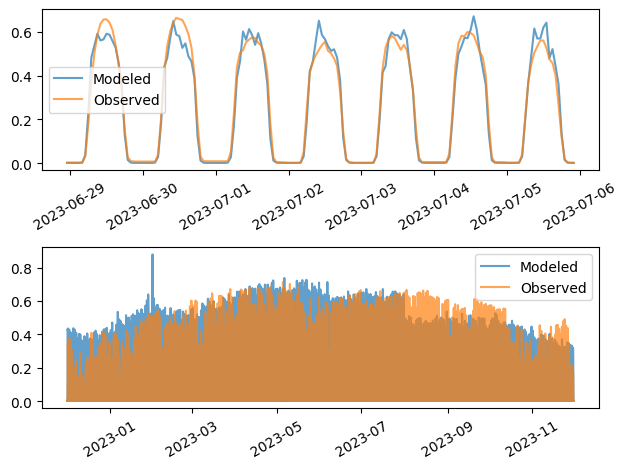
\includegraphics[width=0.7\linewidth]{assets/nhits-solar-pv.png}
    \caption{Weekly and yearly predicted and actual solar PV capacity factor for the N-HiTS model}
    \label{fig:nhits-solar-pv}
\end{figure}
Note how the modeled data is much more rugged on an hourly basis, while the actual data follows a much smoother hour to hour pattern. However, this model is still more accurate with that ruggedness than other smoother models like the SARIMAX or the VARMAX.  
On the yearly pattern it can be seen how the model greatly overestimates some extreme positive values and has some sudden drops in capacity factor around august, but the general patterns are maintained. 
\subsection{Solar TH}
For the solar thermal capacity factor series, the results will be shown in the same way as for the \nameref{s:solar-pv-results} section. The two tables showing the metrics' values and the rank of the models will be presented, and they will later be discussed. 

% \newpage
\begin{table}[ht]
    \footnotesize
    \begin{tabular}[l]{r|c|ccc|cc|}
        \toprule
        \textbf{Solar TH} &Benchmark&Regression&SARIMAX&VARMAX&SVM&XGBoost \\ 
        \midrule            
        Cramer von Mises&12.87&239.5&144.6&209.2&93.37&653.9 \\
        KL divergence&0.01016&0.2558&0.1379&1.014&0.4101&4.31 \\
        ACF$_\xi$ distance&0.02488&0.2246&0.1936&0.1826&0.1988&0.2507 \\
        \midrule
        CCMD&0.01117&0.3291&0.1044&0.2151&0.8375&0.3549 \\
        CCF$_\xi^{Solar PV}$ distance&0.01513&0.1008&0.08724&0.223&0.1686&0.2552 \\
        CCF$_\xi^{Wind}$ distance&0.02013&0.08723&0.1107&0.1376&0.1124&0.861 \\
        \midrule
        CVaR$^+$ distance&0.0732&2.869&-0.04785&-0.5135&11.09&-0.8908 \\
        Tail dependence coefficient$^+$&0.3356&0.3676&0.3539&0.2192&0.05479&0.08844 \\
        Return level distance$^+$&0.2928&17.04&-1.004&-0.9157&1.394e+10&-0.8234 \\
        \bottomrule
    \end{tabular}
\end{table}
\begin{table}[ht]
    \footnotesize
    \begin{flushright}
    \begin{tabular}[r]{|ccc|cccc}
        \toprule
        N-BEATS&N-HiTS&TimeMixer&TFT&Informer&FEDFormer&iTransformer  \\
        \midrule            
        134&124.2&251.4&699.1&714.9&495.9&26.38 \\
        0.2427&0.05258&0.9605&0.4706&0.8153&1.35&0.04629 \\
        0.1812&0.5174&0.1061&0.1951&0.4585&0.1844&0.1639 \\
        \midrule
        0.1959&0.4296&0.05632&0.5398&0.5675&0.5183&0.2093 \\
        0.03605&0.1889&0.09468&0.168&0.2716&0.2363&0.07058 \\
        0.118&0.6707&0.07896&0.208&0.5203&0.1325&0.1419 \\
        \midrule
        1.818&-0.1942&-0.6187&5.324&-0.1614&-0.7453&-0.1516 \\
        0.3813&0.05251&0.2192&0&0.09589&0.08904&0.3721 \\
        6.143&-1.018&-0.8051&0.8068&0.0144&-0.8311&-0.3048 \\
        \bottomrule
    \end{tabular}
    \end{flushright}
    \caption{Results of the different models for Solar TH\label{long}}
    \label{table:results-solar-th}
\end{table}
Again, the model rank table will be shown to better interpret these results.

\newpage
\begin{table}[ht]
    \footnotesize
    \begin{tabular}[l]{r|c|ccc|cc|}
        \toprule
        \textbf{Solar TH} &Benchmark&Regression&SARIMAX&VARMAX&SVM&XGBoost \\
        \midrule            
        Cramer von Mises&(1)&(8)&(6)&(7)&(3)&(11) \\
        KL divergence&(1)&(6)&(4)&(11)&(7)&(13) \\
        ACF$_\xi$ distance&(1)&(10)&(7)&(5)&(9)&(11) \\
        \midrule
        CCMD&(1)&(7)&(3)&(6)&(13)&(8) \\
        CCF$_\xi^{Solar PV}$ distance&(1)&(6)&(4)&(10)&(8)&(12) \\
        CCF$_\xi^{Wind}$ distance&(1)&(3)&(4)&(8)&(5)&(13) \\
        \midrule
        CVaR$^+$ distance&(2)&(11)&\textbf{(1)}&(6)&(13)&(9) \\
        Tail dependence coefficient$^+$&(5)&(3)&(4)&(6)&(11)&(10) \\
        Return level distance$^+$&(2)&(12)&(9)&(8)&(13)&(6) \\
        \bottomrule
        Total&(15)&(66)&(42)&(68)&(82)&(93) \\
        \bottomrule
    \end{tabular}
\end{table}
\begin{table}[ht]
    \footnotesize
    \begin{flushright}
    \begin{tabular}[r]{|ccc|cccc}
        \toprule
        N-BEATS&N-HiTS&TimeMixer&TFT&Informer&FEDFormer&iTransformer \\
        \midrule            
        (5)&(4)&(9)&(12)&(13)&(10)&\textbf{(2)} \\
        (5)&(3)&(10)&(8)&(9)&(12)&\textbf{(2)} \\
        (4)&(13)&\textbf{(2)}&(8)&(12)&(6)&(3) \\
        \midrule
        (4)&(9)&\textbf{(2)}&(11)&(12)&(10)&(5) \\
        \textbf{(2)}&(9)&(5)&(7)&(13)&(11)&(3) \\
        (6)&(12)&\textbf{(2)}&(10)&(11)&(7)&(9) \\
        \midrule
        (10)&(5)&(7)&(12)&(4)&(8)&(3) \\
        \textbf{(1)}&(12)&(6)&(13)&(8)&(9)&(2) \\
        (11)&(10)&(4)&(5)&\textbf{(1)}&(7)&(3) \\
        \bottomrule
        (48)&(77)&(48)&(86)&(83)&(80)&\textbf{(32)} \\
        \bottomrule
    \end{tabular}
    \end{flushright}
    \caption{Results of the rank of the different models for Solar TH\label{long}}
    \label{table:results-rank-solar-pv}
\end{table}

The first thing that should be taken into account before analyzing these results is that the solar thermal series is very similar to the solar photovoltaic series, therefore similar results should be expected. The only difference being more variability at night and higher dependence on previous values of the cross series, mainly of solar photovoltaic. 

Perhaps because of these characteristics there seems to be quite a difference in performance among the top models compared to solar PV. In this case, the iTransformer is clearly the best model. This model is clearly the best in modeling the general distribution of the data, but also does incredibly well in modeling extreme values and quite well on the multivariate characteristics. This could be explained by the fact that the solar thermal series as explained has somewhat of a more complex relationship with lagged values and solar PV and wind values. Thanks to its ability to be stored, its capacity factor is no longer exclusively reliant on weather conditions but also depends on human decisions. That is human decisions that could be affected by how much energy has been stored -- highly correlated with past solar PV data -- and how much has been or is expected to be produced by the rest of the energy resources. As for the rest of the transformer models, they strongly underperform, only doing comparatively better in extreme value modeling, perhaps again due to being able to capture the complex relationships between these extreme values and past or cross values. 

Another surprising part is the drop in performance by the N-HiTS, perhaps due to the higher complexity in this series in the lesser significance of the frequency structure leveraged by this model. The TimeMixer and N-BEATS on the other hand remain really strong performers tying at third place among all models. These models are specially good in capturing the cross relationships between this series and the other two. The TimeMixer model is specially good at this and at capturing the temporal self consistency of the series, while it is not nearly as good in capturing the general distribution of the data.

Among the statistical models the analysis is very similar to solar PV, with the SARIMAX model being again the best within this family and one of the best overall, with the other two models performing significantly worse. 

Regarding the ML models a behaviour similar to the last one is observed, with both doing really poorly although slightly better for the SVM, with the only category where XGBoost does better being the extreme value modeling. This is coherent with what has been observed for the transformer models, where models with more parameters capable of capturing more complex patterns but more prone to overfitting do comparatively better in this evaluation category. 

Below the same representation as before is given but in this case for the iTransformer model, given how this one is the best in this case.
\begin{figure}[ht]
    \centering
    \captionsetup{justification=centering}
    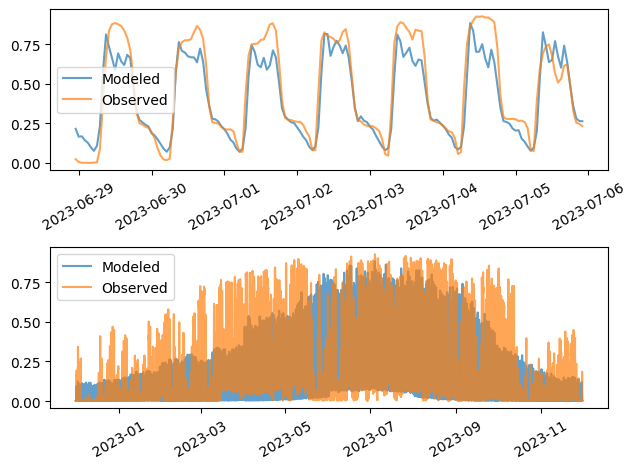
\includegraphics[width=0.7\linewidth]{assets/itransformer-solar-th.png}
    \caption{Weekly and yearly predicted and actual solar TH capacity factor for the iTransformer model}
    \label{fig:itransformer-solar-th}
\end{figure}
In this case, the same ruggedness problem can be seen, which is common to all NN and transformer based models. However, the solar thermal series is not as smooth as the solar photovoltaic so it does not stand as much. It can also be seen how the model accurately models the nightime generation for solar thermal. 
As for the yearly pattern, the model seems to greatly underestimate generation during the winter months and it also assumes a much more uniform generation profile than the real one. 
\subsection{Wind}
The last of the three series is the most different compared to the other two, given the much lower seasonality in wind production and its higher degree of dependence on past cross series. The results obtained for the wind series are the following. Note how in this case both the positive and negative extreme values hold some interest as the lower end of the distribution is no longer zero. In fact, moments of very low wind generation are of special interest given these are the moments when the rest of the energy sources would have to step up.  

\newpage
\begin{table}[ht]
    \footnotesize
    \begin{tabular}[l]{r|c|ccc|cc|}
        \toprule
        \textbf{Wind} &Benchmark&Regression&SARIMAX&VARMAX&SVM&XGBoost \\ 
        \midrule            
        Cramer von Mises&9.483&1783&1814&360.4&434.2&774.6 \\
        KL divergence&0.001479&1.109&1.208&0.1067&0.1318&0.3214 \\
        ACF$_\xi$ distance&0.06016&0.3458&0.3143&0.4598&0.3302&0.6625 \\
        \midrule
        CCMD&0.01117&0.3291&0.1044&0.2151&0.8375&0.3549 \\
        CCF$_\xi^{Solar PV}$ distance&0.01282&0.1621&0.1686&0.05547&0.115&0.4045 \\
        CCF$_\xi^{Solar TH}$ distance&0.01363&0.242&0.2763&0.0691&0.0808&0.525 \\
        \midrule
        CVaR$^+$ distance&-0.02357&0.4225&0.06328&-0.03603&0.02966&-0.5748 \\
        CVaR$^-$ distance&-0.2462&5.582&6.485&3.104&2.912&5.746 \\
        Tail dependence coefficient$^+$&0.04795&0.09132&0.1256&0.1301&0.1119&0.05028 \\
        Tail dependence coefficient$^-$&0.1507&0.1027&0.1553&0.1484&0.05023&0.05003 \\
        Return level distance$^+$&1.362&-0.4957&-0.4707&-0.5817&-0.5813&-1.081 \\
        Return level distance$^-$&-13.51&-7.643&-8.188&-4.958&-3.629&-5.709 \\
        \bottomrule
    \end{tabular}
\end{table}
\begin{table}[ht]
    \footnotesize
    \begin{flushright}
    \begin{tabular}[r]{|ccc|cccc}
        \toprule
        N-BEATS&N-HiTS&TimeMixer&TFT&Informer&FEDFormer&iTransformer  \\
        \midrule            
        381.2&504&553.8&729.6&1283&236&309.9 \\
        0.4356&0.2818&0.2442&0.3298&0.6615&0.1116&0.1838 \\
        0.2918&0.4957&0.2992&0.3452&0.5537&0.3348&0.3312 \\
        \midrule
        0.1959&0.4296&0.05632&0.5398&0.5675&0.5183&0.2093 \\
        0.03014&0.03572&0.04976&0.3294&0.4744&0.03619&0.1731 \\
        0.1954&0.7625&0.06438&0.4002&0.7358&0.03586&0.2802 \\
        \midrule
        -0.5646&-0.504&-0.3975&-0.5549&-0.1147&0.5273&-0.395 \\
        2.788&4.813&3.941&5.036&4.858&0.7204&3.297 \\
        0.09132&0.105&0.08904&0.05479&0.02727&0.02968&0.07534 \\
        0.1119&0.1005&0.09589&0.05251&0.1005&0.04795&0.1872 \\
        -0.8006&-0.9889&-0.8401&-0.9307&-0.4494&0.7511&-0.786 \\
        -2.105&-1.986&-5.443&-6.162&-6.413&-0.6112&-1.679 \\
        \bottomrule
    \end{tabular}
    \end{flushright}
    \caption{Results of the different models for Wind\label{long}}
    \label{table:results-wind}
\end{table}

The rank of each of the models can be seen in \autoref{table:results-rank-wind}. Note how in this case, since both the upper and lower extreme metrics are evaluated, the weight of the extreme value metrics in the total rank will be higher and can skew the percieved overall performance of the models when using this metric.

\newpage
\begin{table}[ht]
    \footnotesize
    \begin{tabular}[l]{r|c|ccc|cc|}
        \toprule
        \textbf{Wind} &Benchmark&Regression&SARIMAX&VARMAX&SVM&XGBoost \\
        \midrule            
        Cramer von Mises&(1)&(12)&(13)&(4)&(6)&(10) \\
        KL divergence&(1)&(12)&(13)&\textbf{(2)}&(4)&(8) \\
        ACF$_\xi$ distance&(1)&(9)&(4)&(10)&(5)&(13) \\
        \midrule
        CCMD&(1)&(7)&(3)&(6)&(13)&(8) \\
        CCF$_\xi^{Solar PV}$ distance&(1)&(8)&(9)&(6)&(7)&(12) \\
        CCF$_\xi^{Solar TH}$ distance&(1)&(7)&(8)&(4)&(5)&(11) \\
        \midrule
        CVaR$^+$ distance&(1)&(8)&(4)&(3)&\textbf{(2)}&(13) \\
        CVaR$^-$ distance&(1)&(11)&(13)&(5)&(4)&(12) \\
        Tail dependence coefficient$^+$&(11)&(6)&(2)&\textbf{(1)}&(3)&(10) \\
        Tail dependence coefficient$^-$&(3)&(6)&(2)&(4)&(11)&(12) \\
        Return level distance$^+$&(13)&(3)&(2)&(5)&(4)&(12) \\
        Return level distance$^-$&(13)&(11)&(12)&(6)&(5)&(8) \\
        \bottomrule
        Total&(48)&(100)&(85)&\textbf{(56)}&(69)&(129) \\
        \bottomrule
    \end{tabular}
\end{table}
\begin{table}[ht]
    \footnotesize
    \begin{flushright}
    \begin{tabular}[r]{|ccc|cccc}
        \toprule
        N-BEATS&N-HiTS&TimeMixer&TFT&Informer&FEDFormer&iTransformer \\
        \midrule            
        (5)&(7)&(8)&(9)&(11)&\textbf{(2)}&(3) \\
        (10)&(7)&(6)&(9)&(11)&(3)&(5) \\
        \textbf{(2)}&(11)&(3)&(8)&(12)&(7)&(6) \\
        \midrule
        (4)&(9)&\textbf{(2)}&(11)&(12)&(10)&(5) \\
        \textbf{(2)}&(3)&(5)&(11)&(13)&(4)&(10) \\
        (6)&(13)&(3)&(10)&(12)&\textbf{(2)}&(9) \\
        \midrule
        (12)&(9)&(7)&(11)&(5)&(10)&(6) \\
        (3)&(8)&(7)&(10)&(9)&\textbf{(2)}&(6) \\
        (6)&(4)&(7)&(9)&(13)&(12)&(8) \\
        (5)&(8)&(9)&(10)&(8)&(13)&\textbf{(1)} \\
        (8)&(11)&(9)&(10)&\textbf{(1)}&(6)&(7) \\
        (4)&(3)&(7)&(9)&(10)&\textbf{(1)}&(2) \\
        \bottomrule
        (66)&(92)&(73)&(117)&(116)&(72)&(68) \\
        \bottomrule
    \end{tabular}
    \end{flushright}
    \caption{Results of the rank of the different models for Wind\label{long}}
    \label{table:results-rank-wind}
\end{table}

At a quick glance it can be seen how the results for the wind series are quite different to those of the other two series. In this case, a different transformer based model -- the FEDFormer -- is the best performer. However, this overall result is highly skewed by the extreme value prediction metric, wehre this model does greatly. In the rest of the categories it also does quite good but not comparatively as much. The iTransformer on the other hand drops quite a few positions in the overall ranking, doing not very badly but not being nearly as dominant, with the general distribution being its best category. The TFT and the Informer are again some of the worst performing models. 

In this case, the VARMAX is surprisingly the best model. It is the first series in which this model outperforms the SARIMAX model, most surely due to the integration component not being significant in this series due to its much higher stationarity. The results of the whole statistical category are however quite surprising, as it would seem by looking at the VARMAX that the simplicity of the model were an advantage, preventing it from capturing spurious patterns more present in the wind series. However, the other two simple models are significantly worse performers. 

Another model with a great improvement in performance is the SVM, for the first time ranking among the top models although not standing out specially in any given category. Again, the XGBoost is the worst performing model.

The N-BEATS and TimeMixer models are again doing very good, with the N-HiTS maintining its drop in performance in this complex series. 

As for the transformers, it would seem like they could maybe benefit from their long run complex pattern capabilities for this series, however as it has already been seen in this series simplicity seems to be the way to go. The iTransformer is agian the best out of all transformer based models, followed by the FEDFormer. This latter model is specially good at modelling the lower tail of the distribution. Although it does significantly worse for the upper tail. 

One final difference for this series is how worse all models are compared to the benchmark relatively to the other two series. No matter what metric one looks at, the gap between the best model and the benchmark is significnatly higher than for the other two series, hinting at the existence of unexploited patterns or modeling criteria that are not being leveraged and that thus do not allow the models to represent the wind series as realistically. 

Finally, regarding the evaluation method itself, it is worth noting how for example all of the models including the benchmark have a very significant negative Return level distance $^-$. What this is showing is that the return level for the lower tail is greately underestimated by all models. If all models including the benchmark show the same bias, it could show that there may be a problem with the data used for evaluation itself, where the lower tail distribution was not representative and thus was underestimated by all models.

\begin{figure}[ht]
    \centering
    \captionsetup{justification=centering}
    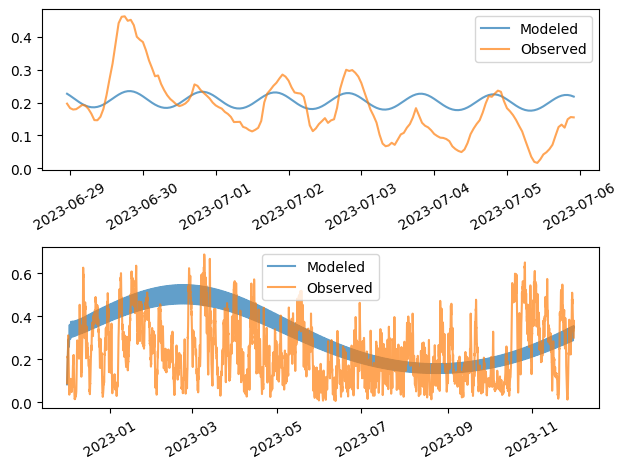
\includegraphics[width=0.7\linewidth]{assets/varmax-wind.png}
    \caption{Weekly and yearly predicted and actual wind capacity factor for the VARMAX model}
    \label{fig:varmax-wind}
\end{figure}
The comparison seen in \autoref{fig:varmax-wind} is by far the most discouraging one. It can be seen how the modeled profile distribution has nothing to do with the actual one. The volatility in the modeled data is much lower than the real one, with all of the data being concentrated around a yearly seasonality which only captures very basic yearly and daily profiles -- with the daily ones being present only in the summer, but the model showing them for the whole year. 

It is not very promising that this is the best model that could be found, although using other models not as constrained by the seasonality and simplicity of the VARMAX does not shed much improvement as seen in \autoref{fig:varmax-nbeats-wind}. 

\begin{figure}[ht]
    \centering
    \captionsetup{justification=centering}
    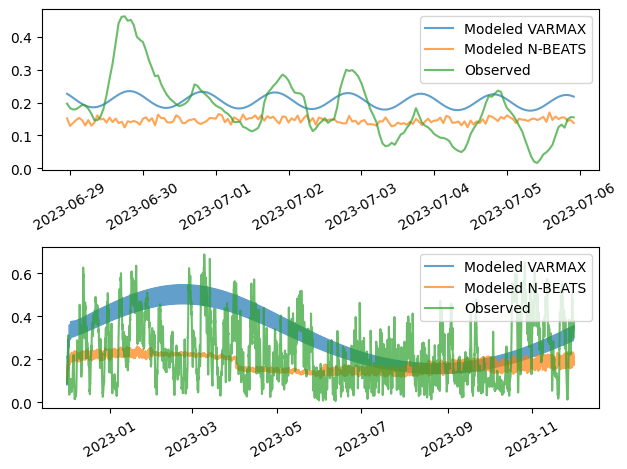
\includegraphics[width=0.7\linewidth]{assets/varmax-nbeats-wind.png}
    \caption{Weekly and yearly predicted and actual wind capacity factor for the VARMAX and N-BEATS model}
    \label{fig:varmax-nbeats-wind}
\end{figure}

This does shed some light on some necessary changes for future works. It is clear that the wind capacity factor has a really prominent random component and a low signal to noise ratio. The loss functions that have been used, which are mainly MAE and SE as they are the standard for these type of tasks, make the model extremely risk averse in their predictions and when they cannot accurately predict the wind values they end up predicting a kind of mean. For more realistic modeling of wind data it seems like different loss functions that don't penalize point errors that much need to be used. 

\subsection{Custom loss function}
After having analyzed the results for all models in the three capacity factor series, it is now time to analyze the results regarding the hypothesis of the custom loss function. That is, can the behaviour of the model be steered through a custom loss function -- in this case the SERA loss -- to better predict extreme values? As explained in the \nameref{s:loss-function} section, an XGBoost model has been trained using this loss function with the same hyperparameters as the base XGBoost model. In fact, two such models have been implemented, one focusing on the upper tail extreme values and one focusing on the lower tail extreme values. The relevance function in both cases has been to give a relevance of 1 to the top or bottom 10\%, a relevance of 0 to the opposite 10\% and the rest of the distribution is given a relevance based on the spline interpolation. 

Note that the modeling has been done using the custom loss only for the wind modeling, given this is the series where there is a highest practical interest to accurately predict extreme events. The results are as follows. 

\newpage
\begin{table}[ht]
    \centering
    \footnotesize
    \begin{tabular}[r]{r|c|cc}
        \toprule
        \textbf{Wind}&XGBoost&XGBoost$^-$&XGBoost$^+$ \\
        \midrule            
        Cramer von Mises&774.6&1332&1978 \\
        KL divergence&0.3214&0.6029&1.678 \\
        ACF$_\xi$ distance&0.6625&0.6622&0.2574 \\
        \midrule
        CCMD&0.3549&0.3584&0.4519 \\
        CCF$_\xi^{Solar PV}$ distance&0.4045&0.3901&0.3306 \\
        CCF$_\xi^{Solar TH}$ distance&0.525&0.5031&0.4071 \\
        \midrule
        CVaR$^+$ distance&-0.5748&-0.4043&-0.235 \\
        CVaR$^-$ distance&5.746&8.46&11.03 \\
        Tail dependence coefficient$^+$&0.05028&0.05008&0.05974 \\
        Tail dependence coefficient$^-$&0.05003&0.04982&0.01963 \\
        Return level distance$^+$&-1.081&-1.206&-0.81 \\
        Return level distance$^-$&-5.709&-6.974&-8.092 \\
        \bottomrule
    \end{tabular}
    \caption{Results of the XGBoost models with SERA loss functions for Wind\label{long}}
    \label{table:results-custom-loss}
\end{table}

Even though these results are much easier to read and interpret than the ones where all of the models are included, the rank will still be provided in order to help interpret the results as much as possible. 

\begin{table}[ht]
    \centering
    \footnotesize
    \begin{tabular}[r]{r|c|cc}
        \toprule
        \textbf{Wind}&XGBoost&XGBoost$^-$&XGBoost$^+$ \\
        \midrule            
        Cramer von Mises&\textbf{(1)}&(2)&(3) \\
        KL divergence&\textbf{(1)}&(2)&(3) \\
        ACF$_\xi$ distance&(3)&(2)&\textbf{(1)} \\
        \midrule
        CCMD&\textbf{(1)}&(2)&(3) \\
        CCF$_\xi^{Solar PV}$ distance&(3)&(2)&\textbf{(1)} \\
        CCF$_\xi^{Solar TH}$ distance&(3)&(2)&\textbf{(1)} \\
        \midrule
        CVaR$^+$ distance&(3)&(2)&\textbf{(1)} \\
        CVaR$^-$ distance&\textbf{(1)}&(2)&(3) \\
        Tail dependence coefficient$^+$&(2)&(3)&\textbf{(1)} \\
        Tail dependence coefficient$^-$&\textbf{(1)}&(2)&(3) \\
        Return level distance$^+$&(2)&(3)&\textbf{(1)} \\
        Return level distance$^-$&\textbf{(1)}&(2)&(3) \\
        \bottomrule
        Total&\textbf{(22)}&(26)&(24) \\
        \bottomrule
    \end{tabular}
    \caption{Results of the XGBoost models' rank with SERA loss functions for Wind\label{long}}
    \label{table:results-rank-custom-loss}
\end{table}

The first insight that can be obtained from these results is that, unsurprisingly, the unbiased XGBoost model seems to be the one best representing the general distribution of the series. This is to be expected as the other two models will probably have introduced some bias in order to better fit extreme values. However, what is surprising is how the upper tail focused model performs better in all metrics regarding temporal consistency both for the series with itself and with the other two series. This probably means that higher wind capacity factor values are more realted to previous wind and solar values than the lower ones. 

Interestingly, this holds not only for the self temporal correlation but also for the cross temporal correlation, with this model being the also the best one regarding the correlation of the wind values with lagged values of the other two series. 

Regarding extreme values, which is actually the whole purpose of introducing the custom loss function, a couple interesting observations can be made. Introducing the SERA loss seems to correctly steer the model into correctly modeling the upper tail of the wind capacity factor. However, this result cannot be replicated for the lower tail and the unbiased model is actually the one with the best performance in the lower extreme values. 